本文探讨的主要内容包括固定翼姿态控制,飞行向导及自主导航等功能,
以层次化的观点来看,PX4由两个层次组成:一是飞行控制栈(flight stack),即自驾仪的软件解决方案,二是中间件,一种可以支持任意类型自主机器人的通用机器人中间件。
如图\ref{px4}所示。整个系统是反应式的。
箭头显示了模块之间最重要的连接的信息流。 实际上,连接比所示的多得多,并且大多数模块都可以访问一些特定的数据(例如,用于参数)。
模块通过使用名为uORB的发布-订阅消息总线相互通信,
使用“发布-订阅”方案意味着:系统是被动的,它是异步的,在有新数据可用时将立即更新
所有操作和通讯都完全并行化, 系统组件可以以线程安全的方式从任何地方使用数据.
其中,uORB(Micro Object Request Broker,微对象请求代理器)是PX4/Pixhawk系统中非常重要且关键的一个模块,它肩负了整个系统的数据传输任务,所有的传感器数据、GPS、PPM信号等都要从芯片获取后通过uORB进行传输到各个模块进行计算处理。实际上uORB是一套跨「进程」 的IPC通讯模块。在Pixhawk中,所有的功能被独立以进程模块为单位进行实现并工作。而进程间的数据交互就由为重要,必须要能够符合实时、有序的特点。

\begin{figure}
    \centering
    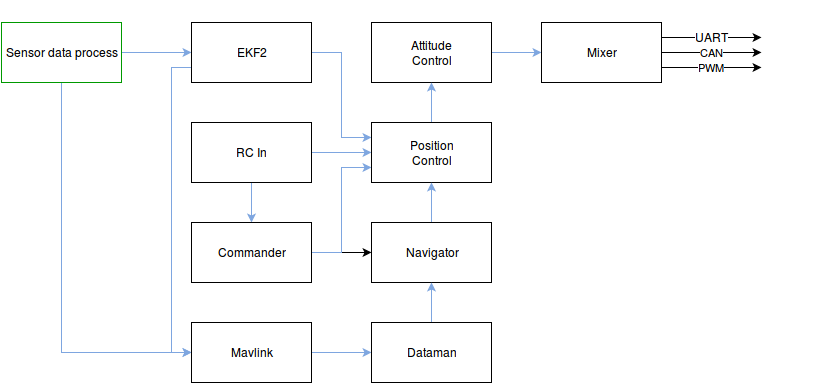
\includegraphics[width=0.5\textwidth]{pictures/PX4_Architecture_1.png}
    \caption{PX4}
    \label{px4}
\end{figure}
   
    其中, 飞行控制栈是用于自主无人机的制导,导航和控制算法的集合。 
    它包括用于固定翼,多旋翼和VTOL机身的控制器,以及用于姿态和位置的估计器。
图\ref{fight}显示了飞行堆栈的构建块的概述。它包含从传感器、RC输入和自动飞行控制(导航器)到电动机或伺服控制(执行器)的完整管道。
\begin{figure}[H]
    \centering
    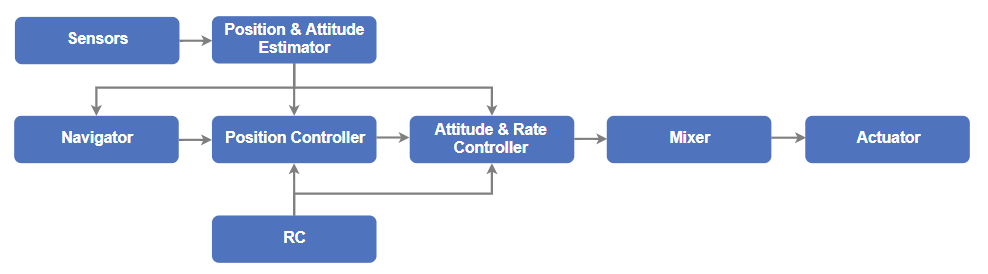
\includegraphics[width=0.6\textwidth]{pictures/fight_stack.png}
    \caption{fight stack}
    \label{fight}
\end{figure}
其中,estimator、controller 和 mixer 担当主要角色。
estimator 获取一个或多个传感器输入,对其进行组合,然后计算vehicle状态(例如,来自IMU传感器数据的姿态);
controller 是将设定值和测量或估计状态(过程变量)作为输入的组件,其目标是调整过程变量的值,使其与设定值匹配,输出是最终达到该设定点的校正。例如,位置控制器将位置设定值作为输入,过程变量是当前估计的位置,输出是将vehicle移向所需位置的姿态和推力设定点;
mixer 接受力指令(例如向右转)并将其转换为单独的电机指令,同时确保不超出某些限制,这种转换是特定于vehicle类型的,并且取决于各种因素,例如相对于重心的电动机布置或vehicle的旋转惯性。
本文主要对 controller 内部的算法进行了一定的改进。\par
控制器主要包括:导航控制器(navigator)、制导控制器(position controller)和姿态控制器(attitude controller)三层结构;同时,上层的输出也是下层的输入,之间紧密衔接,没有主次之分。